\documentclass[
	12pt,				      % tamanho da fonte
	openright,			      % capítulos começam em pág ímpar (insere página vazia caso preciso)
	oneside,			      % para impressão apenas no anverso (se quiser frente e verso, mude para twosi   
	a4paper,			      % tamanho do papel
	english,			      % idioma adicional para hifenização
	brazilian,  		      % o último idioma é o principal do documento
    chapter=TITLE,            % títulos de capítulos convertidos em letras maiúsculas
    section=TITLE,            % títulos de seções convertidos em letras maiúsculas
    subsection=TITLE,         % títulos de subseções convertidos em letras maiúsculas
    subsubsection=TITLE,      % títulos de subsubseções em letras maiúsculas
    subsubsubsection=TITLE,   % títulos de subsubsubseções em letras maiúsculas
	]{abntex2}

% ---
% Importação de pacotes de configurações e preâmbulo
% ---

% --------------------------------------------------
% CONFIGURAÇÃO DE FONTES (XeLaTeX)
% --------------------------------------------------

%\usepackage{fontspec}



% Utiliza Times New Roman quando disponível.
% Caso contrário (ex.: Overleaf), utiliza TeX Gyre Termes.

%\setmainfont{Times New Roman}
%\setmainfont{TeX Gyre Termes}
\usepackage{newtxtext} % Fonte times new romam no texto
\usepackage{newtxmath}
%\usepackage{textcase}
%\renewcommand{\ABNTEXchapterfont}{\rmfamily\bfseries} % Fonte times new romam em negrito nos itens



% --------------------------------------------------
% AJUSTE DE TAMANHO DE FONTES DOS TÍTULOS (Conforme Manual IFPI)
% --------------------------------------------------
\renewcommand{\ABNTEXchapterfont}{\rmfamily\bfseries}
\renewcommand{\ABNTEXchapterfontsize}{\normalsize}

% Força tamanho 12pt para títulos de seções
\renewcommand{\ABNTEXsectionfont}{\rmfamily}
\renewcommand{\ABNTEXsectionfontsize}{\normalsize}

% Força tamanho 12pt para títulos de subseções
\renewcommand{\ABNTEXsubsectionfont}{\bfseries}
%\renewcommand{\tocheadstart}{\ABNTEXsubsectionfont}{\bfseries}
\renewcommand{\ABNTEXsubsectionfontsize}{\normalsize}

% Força tamanho 12pt para títulos de subsubseções
\renewcommand{\ABNTEXsubsubsectionfont}{\rmfamily\bfseries}
\renewcommand{\ABNTEXsubsubsectionfontsize}{\normalsize}

% Força tamanho 12pt para títulos de subsubsubseções (se usar)
\renewcommand{\ABNTEXsubsubsubsectionfont}{\rmfamily\bfseries}
\renewcommand{\ABNTEXsubsubsubsectionfontsize}{\normalsize}



% --------------------------------------------------
% PACOTES GERAIS
% --------------------------------------------------

\usepackage{indentfirst}
\usepackage{xcolor}
\usepackage{graphicx}
\usepackage{microtype}
\usepackage{lipsum}
\usepackage{amsmath}
\usepackage{booktabs}
\usepackage{listings}
\usepackage{float}
\usepackage{caption}
\usepackage{csquotes}

% --------------------------------------------------
% CONFIGURAÇÃO DO LISTINGS
% --------------------------------------------------

\lstset{
	basicstyle=\ttfamily\footnotesize,
	breaklines=true,
	frame=single,
	numbers=left,
	numberstyle=\tiny,
	captionpos=b,
	keepspaces=true,
	showstringspaces=false,
	tabsize=4
}

% --------------------------------------------------
% BIBLATEX
% --------------------------------------------------

\usepackage[
backend=biber,
style=abnt,
justify=true,
sorting=nty
]{biblatex}

\addbibresource{referencias.bib}

% --------------------------------------------------
% HIPERLINKS
% --------------------------------------------------

\definecolor{blue}{RGB}{41,5,195}

\makeatletter

\hypersetup{
	pdftitle={\@title},
	pdfauthor={\@author},
	pdfsubject={\imprimirpreambulo},
	pdfcreator={LaTeX with abnTeX2},
	pdfkeywords={abnt,latex,abntex,abntex2,relatório técnico},
	colorlinks=true,
	linkcolor=black,
	citecolor=black,
	filecolor=magenta,
	urlcolor=blue,
	bookmarksdepth=4
}

\makeatother

% --------------------------------------------------
% PARÁGRAFOS
% --------------------------------------------------

\setlength{\parindent}{1.25cm}
\setlength{\parskip}{0pt}

% --------------------------------------------------
% ÍNDICE
% --------------------------------------------------

\makeindex

% --------------------------------------------------
% COMANDO PARA FONTE DE FIGURAS E TABELAS
% --------------------------------------------------

\newcommand{\source}[1]{%
	\vspace{0.2cm}
	\par
	\noindent
	\textbf{Fonte:} #1
}

% --------------------------------------------------
% AMBIENTE QUADRO (necessário para \listadequadros)
% --------------------------------------------------

\usepackage{newfloat}

\DeclareFloatingEnvironment[
fileext=loq,
listname={Lista de Quadros},
name=Quadro,
placement=htbp
]{quadro}

\captionsetup[quadro]{position=top}
\captionsetup[quadro]{justification=centering}
\captionsetup[quadro]{font=normalfont}
\captionsetup[quadro]{labelfont=bf}

\newcommand{\listadequadros}{
    \pdfbookmark[0]{\listquadroname}{loq}
    \listof{quadro}{\listquadroname}
}


% ---
% DADOS DE IDENTIFICAÇÃO DO TRABALHO
% ---

% Título do trabalho
\titulo{TÍTULO DO TRABALHO: Subtítulo (se houver)}
\newcommand{\titulorosto}{TÍTULO DO TRABALHO: Subtítulo (se houver)}

% Nome do Autor(a)
\autor{NOME COMPLETO DO(A) ALUNO(A)}

% Matrícula do aluno (comando customizado)
%\newcommand{\matricula}{202X1TADS0000}

% Local e Data
\local{\textbf{ANGICAL DO PIAUÍ -- PI}}
\data{\textbf{2026}}
\newcommand{\localrosto}{ANGICAL DO PIAUÍ -- PI}
\newcommand{\datarosto}{2026}

% Orientador e Coorientador
\orientador{Prof. Titulação Nome do Orientador}
\coorientador{Prof. Titulação Nome do Coorientador (se houver)}

% Instituição
\instituicao{%
  INSTITUTO FEDERAL DE EDUCAÇÃO, CIÊNCIA E TECNOLOGIA DO PIAUÍ -- IFPI
  \par
  CAMPUS ANGICAL
  \par
    CURSO SUPERIOR DE TECNOLOGIA EM ANÁLISE E DESENVOLVIMENTO DE SISTEMAS}

% Natureza do trabalho (Preâmbulo)
\tipotrabalho{Relatório Técnico de Software (RTS)}

% Data de aprovação (apresentação do TCC)
\newcommand{\dataaprova}{XX/XX/XXXX}

\preambulo{Relatório Técnico de Software apresentado ao Curso Superior de Tecnologia em Análise e Desenvolvimento de Sistemas do Instituto Federal de Educação, Ciência e Tecnologia do Piauí -- Campus Angical, como requisito parcial para a obtenção do título de Tecnólogo em Análise e Desenvolvimento de Sistemas. }

% ---
% CUSTOMIZAÇÃO DA CAPA (para atender às diretrizes do PPC)
% ---
% ---
% CUSTOMIZAÇÃO DA CAPA (para atender às diretrizes do PPC e Manual IFPI)
% ---
\renewcommand{\imprimircapa}{%
	\begin{capa}%
		\center
		
		% Inserção do Logo do IFPI
		% Certifique-se de ter o arquivo logo-ifpi.png (ou .jpg/.pdf) na mesma pasta ou na pasta de imagens
		
\includegraphics[width=3.5cm]{logo-ifpi.png} % Ajuste a largura conforme necessário
		\vspace{0.5cm} % Espaçamento entre o logo e o nome da instituição
		
		% Nome da instituição (tamanho 12pt = \normalsize)
		{\ABNTEXchapterfont\normalsize\imprimirinstituicao}
		
		\vspace*{3cm}
		
		% Nome do autor (tamanho 12pt)
		{\ABNTEXchapterfont\normalsize\imprimirautor}
		
		%\vspace*{1cm}
		
		% Matrícula (tamanho 12pt)
		%{\normalsize Matrícula: \matricula}
		
		%\vfill
		\vspace*{3cm}
		\begin{center}
			% Título do trabalho (tamanho 12pt, negrito)
			\ABNTEXchapterfont\bfseries\normalsize\imprimirtitulo
		\end{center}
		\vfill
		
		% Local e Data (tamanho 12pt)
		\normalsize\imprimirlocal\par
		\normalsize\imprimirdata
		
		\vspace*{1cm}
	\end{capa}
}

% ---
% CUSTOMIZAÇÃO DA FOLHA DE ROSTO
% ---
\renewcommand{\imprimirfolhaderosto}{%
	\begin{folhaderosto}%
		\center
		
		% Nome do aluno (centralizado, tamanho 12pt)
		{\normalsize\imprimirautor}
		
		\vspace*{3cm}
		
		% Título do trabalho (centralizado, tamanho 12pt, negrito)
		{\normalsize\titulorosto}
		
		\vspace*{2cm}
		
		% Bloco da natureza do trabalho e orientador
		% Alinhado do meio da mancha gráfica para a margem direita
		\begin{flushright}
			\begin{minipage}{8cm}
				{\normalsize\imprimirpreambulo}
				
				\vspace*{1cm}
				
				{\normalsize Orientador: \imprimirorientador}
                				
				% Descomente a linha abaixo se houver coorientador
				% {\normalsize Coorientador: \imprimircoorientador}
			\end{minipage}
		\end{flushright}
		
		\vspace*{2cm}
		
		% Data de aprovação (alinhada à esquerda)
		%{\normalsize Data de aprovação: \dataaprova}
		
		
		\vfill
		
		% Local e Data (centralizados, tamanho 12pt)
		\center
		{\normalsize\localrosto}
		
		{\normalsize\datarosto}
		
		\vspace*{1cm}
	\end{folhaderosto}
}


% ---
% Início do documento
% ---
\begin{document}

% Seleciona o idioma do documento (por padrão, o último passado na classe)
\selectlanguage{brazil}

% Retira espaço extra obsoleto entre as frases
\frenchspacing 

% ----------------------------------------------------------
% ELEMENTOS PRÉ-TEXTUAIS
% ----------------------------------------------------------
\pretextual

% Capa (customizada no preambulo.tex)
\imprimircapa

% Folha de rosto (com ficha catalográfica no verso)
%\imprimirfolhaderosto

% Inserir folha de aprovação (descomente após a defesa)
%% ----------------------------------------------------------
% FOLHA DE APROVAÇÃO
% ----------------------------------------------------------

\begin{folhadeaprovacao}

\begin{center}

{\ABNTEXchapterfont\bfseries\imprimirautor}

\vspace{2cm}

{\ABNTEXchapterfont\bfseries\imprimirtitulo}

\vspace{2cm}

\end{center}

\begin{flushright}
	\begin{minipage}{8cm}
		{\normalsize\imprimirpreambulo}
				
	\end{minipage}
\end{flushright}




%Relatório Técnico de Software apresentado ao Curso Superior de Tecnologia em Análise e Desenvolvimento de Sistemas do Instituto Federal de Educação, Ciência e Tecnologia do Piauí -- Campus Angical, como requisito parcial para a obtenção do título de Tecnólogo em Análise e Desenvolvimento de Sistemas.

\vspace{0.5cm}

Área de concentração: Tecnologia da Informação.

\vspace{1cm}

{\normalsize Data de aprovação: \dataaprova}

\vspace{1cm}

\begin{center}
BANCA EXAMINADORA
\end{center}

\vspace{1cm}

\begin{center}

\rule{10cm}{0.4pt}
\par
\imprimirorientador

Instituto Federal do Piauí

Orientador

\vspace{1cm}

\rule{10cm}{0.4pt}

Prof. Dr. Nome do Avaliador 1

Instituto Federal do Piauí

Membro

\vspace{1cm}

\rule{10cm}{0.4pt}

Prof. Me. Nome do Avaliador 2

Instituto Federal do Piauí

Membro

\end{center}

\end{folhadeaprovacao}

% Agradecimentos (para remover, comente a linha abaixo)
% ---
% Agradecimentos
% Este elemento é opcional conforme a ABNT NBR 14724:2024.
% Para remover, comente a linha % ---
% Agradecimentos
% Este elemento é opcional conforme a ABNT NBR 14724:2024.
% Para remover, comente a linha % ---
% Agradecimentos
% Este elemento é opcional conforme a ABNT NBR 14724:2024.
% Para remover, comente a linha \input{capitulos/agradecimentos} no main.tex.
% ---
\begin{agradecimentos}
Dedicamos este template à primeira turma do Curso Superior de Tecnologia em Análise e Desenvolvimento de Sistemas do Instituto Federal de Educação, Ciência e Tecnologia do Piauí -- Campus Angical.

Este documento foi elaborado para padronizar a apresentação dos Relatórios Técnicos, contribuindo para a qualidade e a organização dos trabalhos acadêmicos desenvolvidos no curso.

Registramos nosso reconhecimento aos estudantes, docentes, técnicos administrativos e gestores que contribuíram para a implantação e consolidação deste curso, marco importante na formação de profissionais de tecnologia no IFPI Campus Angical.

\textit{``O futuro pertence àqueles que acreditam na beleza de seus sonhos.''} --- Eleanor Roosevelt
\end{agradecimentos}
 no main.tex.
% ---
\begin{agradecimentos}
Dedicamos este template à primeira turma do Curso Superior de Tecnologia em Análise e Desenvolvimento de Sistemas do Instituto Federal de Educação, Ciência e Tecnologia do Piauí -- Campus Angical.

Este documento foi elaborado para padronizar a apresentação dos Relatórios Técnicos, contribuindo para a qualidade e a organização dos trabalhos acadêmicos desenvolvidos no curso.

Registramos nosso reconhecimento aos estudantes, docentes, técnicos administrativos e gestores que contribuíram para a implantação e consolidação deste curso, marco importante na formação de profissionais de tecnologia no IFPI Campus Angical.

\textit{``O futuro pertence àqueles que acreditam na beleza de seus sonhos.''} --- Eleanor Roosevelt
\end{agradecimentos}
 no main.tex.
% ---
\begin{agradecimentos}
Dedicamos este template à primeira turma do Curso Superior de Tecnologia em Análise e Desenvolvimento de Sistemas do Instituto Federal de Educação, Ciência e Tecnologia do Piauí -- Campus Angical.

Este documento foi elaborado para padronizar a apresentação dos Relatórios Técnicos, contribuindo para a qualidade e a organização dos trabalhos acadêmicos desenvolvidos no curso.

Registramos nosso reconhecimento aos estudantes, docentes, técnicos administrativos e gestores que contribuíram para a implantação e consolidação deste curso, marco importante na formação de profissionais de tecnologia no IFPI Campus Angical.

\textit{``O futuro pertence àqueles que acreditam na beleza de seus sonhos.''} --- Eleanor Roosevelt
\end{agradecimentos}


% Epígrafe (OPCIONAL - para remover, comente a linha abaixo)
%% ---
% Epígrafe
% Este elemento é OPCIONAL conforme a ABNT NBR 14724:2024.
%
% COMO HABILITAR: Mantenha este arquivo como está.
% COMO REMOVER: Comente a linha % ---
% Epígrafe
% Este elemento é OPCIONAL conforme a ABNT NBR 14724:2024.
%
% COMO HABILITAR: Mantenha este arquivo como está.
% COMO REMOVER: Comente a linha % ---
% Epígrafe
% Este elemento é OPCIONAL conforme a ABNT NBR 14724:2024.
%
% COMO HABILITAR: Mantenha este arquivo como está.
% COMO REMOVER: Comente a linha \input{capitulos/epigrafe} no arquivo main.tex.
%
% A epígrafe é uma citação seguida de indicação de autoria, relacionada com
% a matéria tratada no corpo do trabalho. Pode também constar nas folhas ou
% páginas de abertura das seções primárias.
% ---
\begin{epigrafe}
    \vspace*{\fill}
	\begin{flushright}
    \begin{minipage}{9cm}
		\textit{``Qualquer tolo consegue escrever código que um computador entenda.\\
		Bons programadores escrevem código que humanos possam entender.''}\\
		(Martin Fowler)

    \end{minipage}
	\end{flushright}
\end{epigrafe}


 no arquivo main.tex.
%
% A epígrafe é uma citação seguida de indicação de autoria, relacionada com
% a matéria tratada no corpo do trabalho. Pode também constar nas folhas ou
% páginas de abertura das seções primárias.
% ---
\begin{epigrafe}
    \vspace*{\fill}
	\begin{flushright}
    \begin{minipage}{9cm}
		\textit{``Qualquer tolo consegue escrever código que um computador entenda.\\
		Bons programadores escrevem código que humanos possam entender.''}\\
		(Martin Fowler)

    \end{minipage}
	\end{flushright}
\end{epigrafe}


 no arquivo main.tex.
%
% A epígrafe é uma citação seguida de indicação de autoria, relacionada com
% a matéria tratada no corpo do trabalho. Pode também constar nas folhas ou
% páginas de abertura das seções primárias.
% ---
\begin{epigrafe}
    \vspace*{\fill}
	\begin{flushright}
    \begin{minipage}{9cm}
		\textit{``Qualquer tolo consegue escrever código que um computador entenda.\\
		Bons programadores escrevem código que humanos possam entender.''}\\
		(Martin Fowler)

    \end{minipage}
	\end{flushright}
\end{epigrafe}




% Resumo em português
\input{capitulos/resumo}

% Resumo em inglês (Abstract)
%% ---
% Abstract
% ---
\begin{resumo}[Abstract]
 \begin{otherlanguage*}{english}
   This is the english abstract. It should highlight the objective, method, results and conclusions of the document. The order and extent of these items depend on the type of abstract (informative or indicative) and the treatment each item receives in the original document. Keywords should appear just below the abstract, preceded by the expression Keywords:, separated by dot and also finalized by dot.

   \vspace{\onelineskip}
 
   \noindent 
   \textbf{Keywords}: latex; abntex; technical report; software.
 \end{otherlanguage*}
\end{resumo}


% Lista de ilustrações (gerada automaticamente)
\pdfbookmark[0]{\listfigurename}{lof}
\listoffigures*
\cleardoublepage

% Lista de tabelas (gerada automaticamente)
\pdfbookmark[0]{\listtablename}{lot}
\listoftables*
\cleardoublepage
% Lista de quadros (gerada automaticamente)
\listadequadros
\cleardoublepage

% Lista de siglas e abreviaturas
% ---
% Lista de abreviaturas e siglas
% ---
\begin{siglas}
  \item[ABNT] Associação Brasileira de Normas Técnicas
  \item[API] \textit{Application Programming Interface}
  \item[IFPI] Instituto Federal de Educação, Ciência e Tecnologia do Piauí
  \item[PPC] Projeto Pedagógico de Curso
  \item[RTS] Relatório Técnico de Software
  \item[SGBD] Sistema Gerenciador de Banco de Dados
  \item[TADS] Tecnologia em Análise e Desenvolvimento de Sistemas
\end{siglas}


% Sumário (gerado automaticamente)
\pdfbookmark[0]{\contentsname}{toc}
\tableofcontents*
\cleardoublepage

% ----------------------------------------------------------
% ELEMENTOS TEXTUAIS
% ----------------------------------------------------------
\textual

% As seções seguem a estrutura definida pelo PPC do TADS IFPI:
% 1 Introdução | 2 Tecnologias Envolvidas | 3 Modelagem do Projeto
% 4 Software | 5 Considerações Finais

% ---
% 1 Introdução
% Este arquivo contém a seção introdutória do Relatório Técnico de Software.
% Conforme as Diretrizes do PPC, a introdução deve contextualizar o problema,
% apresentar os objetivos e a justificativa do projeto.
% ---
\chapter{Introdução}
\label{cap:introducao}

A gestão de pessoas no serviço público federal envolve processos administrativos complexos, regulamentados por legislação específica que impõe prazos, critérios e fluxos de aprovação rigorosos. Entre esses processos, destaca-se a concessão de Licença Capacitação, prevista no art. 87 da Lei nº 8.112, de 11 de dezembro de 1990, que garante ao servidor público federal o direito de se afastar de suas atividades por até 90 dias a cada quinquênio de efetivo exercício, com a finalidade de participar de ações de desenvolvimento profissional.

Segundo \textcite{pressman_engenharia}, a engenharia de software é uma disciplina que se ocupa de todos os aspectos da produção de software, desde os estágios iniciais de especificação do sistema até a manutenção desse sistema após ele entrar em uso. Nesse contexto, o desenvolvimento de sistemas voltados à automação de processos administrativos representa uma das aplicações mais relevantes dessa disciplina, especialmente em ambientes institucionais onde a conformidade legal é requisito indispensável.

O presente projeto tem como proposta o desenvolvimento de um sistema informatizado para o controle e gerenciamento de solicitações de Licença Capacitação, em substituição ao processo atualmente realizado de forma manual por meio de planilhas eletrônicas e documentos físicos. A solução proposta visa digitalizar e automatizar o fluxo de solicitação, tramitação e concessão da licença, garantindo conformidade com a legislação vigente — em especial o Decreto nº 9.991, de 28 de agosto de 2019, e a Instrução Normativa SGP-ENAP/SEDGG/ME nº 21, de 1º de fevereiro de 2021.

\section{Problema}

O setor responsável pelo gerenciamento de Licença Capacitação da instituição conduz atualmente todo o processo de forma manual, utilizando planilhas eletrônicas e registros físicos para controlar as solicitações dos servidores. Essa abordagem apresenta uma série de problemas operacionais que comprometem a eficiência e a conformidade legal do processo.

\begin{citacao}
A engenharia de software é uma disciplina de engenharia relacionada com todos os aspectos da produção de software, desde os estágios iniciais de especificação do sistema até a manutenção desse sistema, depois que ele entrou em uso. Nessa definição, existem duas frases-chave: disciplina de engenharia e todos os aspectos da produção de software \cite[p.~39]{pressman_engenharia}.
\end{citacao}

Entre os principais problemas identificados no processo atual, destacam-se:

\begin{itemize}
    \item Dificuldade em identificar quais servidores já possuem direito adquirido ao quinquênio de cinco anos de efetivo exercício;
    \item Ausência de controle automatizado sobre conflitos de datas entre solicitações simultâneas;
    \item Falta de rastreabilidade do fluxo de aprovação, tornando difícil identificar em qual etapa uma solicitação se encontra;
    \item Impossibilidade de monitorar em tempo real o limite legal de 5\% de servidores afastados simultaneamente, conforme o art. 27 do Decreto nº 9.991/2019;
    \item Dificuldade no controle do saldo de dias utilizados por servidor em cada quinquênio;
    \item Registro manual e suscetível a erros das parcelas de licença e seus respectivos períodos.
\end{itemize}

Esses problemas resultam em retrabalho, risco de descumprimento da legislação e dificuldade na tomada de decisões pelos gestores responsáveis pelo processo.

\section{Objetivos}

Nesta seção são apresentados os objetivos do projeto, delimitando o escopo do trabalho e orientando as etapas de desenvolvimento e avaliação da solução proposta.

\subsection{Objetivo Geral}

Desenvolver um sistema web para o controle e gerenciamento de solicitações de Licença Capacitação de servidores públicos federais, em conformidade com a Lei nº 8.112/1990, o Decreto nº 9.991/2019 e a Instrução Normativa SGP-ENAP/SEDGG/ME nº 21/2021.

\subsection{Objetivos Específicos}

\begin{itemize}
    \item Realizar o levantamento e a validação dos requisitos de negócio junto aos responsáveis pelo setor, identificando as regras estabelecidas pela legislação vigente;
    \item Modelar o banco de dados relacional para armazenamento e controle das informações de servidores, solicitações, tramitações, licenças e parcelas;
    \item Implementar o módulo de banco de dados com as restrições de integridade que garantam a conformidade legal das operações;
    \item Documentar as regras de negócio que devem ser implementadas no backend, assegurando a divisão correta de responsabilidades entre as camadas do sistema;
    \item Implementar o fluxo de tramitação com as três etapas obrigatórias de aprovação previstas na IN 21/2021: chefia imediata, gestão de pessoas e autoridade máxima;
    \item Realizar testes de validação do sistema junto aos usuários finais do setor responsável.
\end{itemize}

\section{Justificativa}

A automação do processo de controle de Licença Capacitação justifica-se por razões técnicas, legais e operacionais. Do ponto de vista legal, o processo envolve regras específicas estabelecidas pela Lei nº 8.112/1990, pelo Decreto nº 9.991/2019 e pela IN 21/2021, que impõem critérios rigorosos de elegibilidade, prazos, limites de afastamento e fluxos de aprovação. O descumprimento dessas regras pode gerar irregularidades administrativas de responsabilidade da instituição.

Do ponto de vista operacional, a substituição do processo manual por um sistema informatizado reduz significativamente o risco de erros humanos, elimina retrabalho e proporciona rastreabilidade completa de cada solicitação — desde a abertura até a concessão oficial. O sistema permitirá que o setor de gestão de pessoas identifique, em tempo real, quais servidores têm direito à licença, quantos estão afastados simultaneamente e qual é o saldo de dias disponível para cada servidor no quinquênio vigente.

Do ponto de vista acadêmico, o projeto representa a aplicação prática dos conceitos de análise de requisitos, modelagem de banco de dados relacional, normalização e implementação de restrições de integridade referencial, abordados ao longo do Curso Superior de Tecnologia em Análise e Desenvolvimento de Sistemas. A escolha de um problema real, com legislação consolidada e stakeholders identificáveis, confere ao projeto relevância prática e alinhamento com as competências previstas no Projeto Pedagógico do Curso.

Para mais informações sobre a legislação que regulamenta a Licença Capacitação, consulte o Portal da Legislação do Governo Federal: \url{https://www.planalto.gov.br}.

A modelagem do banco de dados será apresentada no Capítulo \ref{cap:modelagem}, enquanto os resultados da implementação serão discutidos no Capítulo \ref{cap:software}.
% ---
% 2 Tecnologias Envolvidas
% Este arquivo descreve as tecnologias utilizadas no projeto.
% Conforme as Diretrizes do PPC, deve-se justificar as escolhas tecnológicas.
% ---
\chapter{TECNOLOGIAS ENVOLVIDAS}
\label{cap:tecnologias}

Neste capítulo, devem ser descritas todas as tecnologias, ferramentas, linguagens de programação, \textit{frameworks} e bibliotecas utilizados no desenvolvimento do projeto. Conforme as Diretrizes do PPC, o objetivo é justificar as escolhas tecnológicas com base em critérios técnicos.

Não se limite a listar as ferramentas; explique o papel de cada uma no contexto da arquitetura do software e os motivos que levaram à sua adoção em detrimento de alternativas disponíveis no mercado.

\section{Linguagens de Programação e Frameworks}

Descreva as linguagens utilizadas no \textit{frontend} e \textit{backend}, bem como os \textit{frameworks} adotados. Por exemplo, justifique o uso de Python com Django para o \textit{backend} devido à sua produtividade \cite{django_docs}, ou React para o \textit{frontend} devido à sua capacidade de criar interfaces reativas.

\section{Banco de Dados}

O Sistema Gerenciador de Banco de Dados (SGBD) escolhido para o desenvolvimento do sistema de Licença Capacitação foi o \textbf{MySQL}, em sua versão estável mais recente. A escolha se justifica principalmente pela necessidade de \textbf{integridade relacional consistente}, uma vez que o domínio do problema é regido por regras legais rígidas oriundas da Lei nº 8.112/1990, do Decreto nº 9.991/2019 e da Instrução Normativa nº 21/2021, que precisam ser refletidas em nível de banco de dados por meio de restrições de integridade (chaves estrangeiras, checagens de unicidade e validações de domínio).

Entre os fatores que motivaram a escolha, destacam-se:

\begin{itemize}
\item \textbf{Suporte a constraints e integridade referencial} (chaves estrangeiras, \texttt{UNIQUE}, \texttt{CHECK}), essencial para impedir, por exemplo, o cadastro de parcelas de afastamento com sobreposição de datas;
\item \textbf{Ampla adoção no mercado e em sistemas do setor público}, o que facilita manutenção futura, contratação de suporte e integração com outras soluções institucionais;
\item \textbf{Boa performance em operações de leitura e escrita}, adequada ao volume de dados esperado para o sistema (cadastro de servidores, solicitações e parcelas de afastamento);
\item \textbf{Gratuidade (Community Edition) e ampla documentação}, adequado ao contexto de um projeto acadêmico sem custos de licenciamento;
\item \textbf{Curva de aprendizado reduzida e ferramental maduro} (MySQL Workbench, phpMyAdmin), o que facilita a modelagem, administração e documentação técnica exigida por este relatório.
\end{itemize}

Optou-se por um modelo estritamente relacional, em detrimento de soluções NoSQL, dado que o domínio da aplicação exige consistência transacional (utilizando o mecanismo de armazenamento InnoDB, que garante conformidade com as propriedades ACID) e relacionamentos bem definidos entre entidades como servidor, solicitação, tramitação e parcela — características para as quais os SGBDs relacionais são mais adequados. Para mais detalhes sobre o MySQL, consulte a documentação oficial \cite{mysql_manual}.

\section{Ferramentas de Desenvolvimento e Controle de Versão}

Para o desenvolvimento do sistema, foram utilizadas as seguintes ferramentas de apoio:

\begin{itemize}
    \item \textbf{IDE/Editor:} \textbf{Visual Studio Code (VS Code)}, utilizado por toda a equipe para o desenvolvimento do backend, frontend e scripts de banco de dados, devido à sua leveza, extensibilidade e suporte nativo a diversas linguagens;
    \item \textbf{Controle de Versão:} \textbf{Git}, associado ao \textbf{GitHub}\footnote{GitHub: \url{https://github.com}} como plataforma de hospedagem remota, permitindo o versionamento colaborativo do código-fonte e o acompanhamento do histórico de alterações entre os membros da equipe;
    \item \textbf{Ferramentas de Modelagem:} \textbf{draw.io}, utilizada na elaboração do Diagrama Entidade-Relacionamento (DER) em notação clássica (retângulos para entidades, elipses para atributos, elipses sublinhadas para chaves primárias e losangos para relacionamentos), apresentado na Seção \ref{cap:modelagem};
    \item \textbf{Validação de Requisitos:} \textbf{Google Forms}, utilizado para a coleta de \textit{feedback} junto às partes interessadas (\textit{stakeholders}) durante a fase de validação das regras de negócio do módulo de banco de dados.
\end{itemize}

% ---
% ATENÇÃO: Este arquivo requer o seguinte pacote no preâmbulo:
% \usepackage{longtable}
% ---
% 3 Modelagem do Projeto
% Este arquivo contém a documentação técnica e modelagem do software.
% Conforme as Diretrizes do PPC, deve incluir: levantamento de requisitos,
% diagrama de casos de uso, diagrama de classes, arquitetura do sistema,
% diagrama entidade-relacionamento e interfaces.
% ---
\chapter{MODELAGEM DO PROJETO}
\label{cap:modelagem}

Este capítulo apresenta a documentação técnica e a modelagem do Sistema de Controle de Licença Capacitação, cobrindo aspectos de engenharia de requisitos, design de interface e modelagem de dados, conforme exigido pelas Diretrizes do PPC. O levantamento de requisitos foi realizado com base na legislação federal vigente — Lei nº 8.112/1990, Decreto nº 9.991/2019 e Instrução Normativa SGP-ENAP/SEDGG/ME nº 21/2021 — e nas necessidades identificadas junto ao setor responsável pelo processo na instituição.

\section{Levantamento de Requisitos}

O levantamento de requisitos foi conduzido por meio de análise da legislação vigente e de entrevistas com os responsáveis pelo setor de gestão de pessoas da instituição. O processo atual, realizado manualmente por meio de planilhas eletrônicas, apresenta problemas como conflitos de datas não detectados, ausência de rastreabilidade do fluxo de aprovação e dificuldade no controle do limite legal de servidores afastados simultaneamente. Os requisitos identificados foram organizados em funcionais e não funcionais, conforme apresentado a seguir.

\subsection{Requisitos Funcionais}
Os Requisitos Funcionais (RF) descrevem o que o sistema deve fazer. A Tabela \ref{tab:requisitos_funcionais} apresenta os requisitos funcionais identificados.

\begin{longtable}{|p{1.8cm}|p{1.8cm}|p{6.5cm}|p{4cm}|}
\caption{Lista de Requisitos Funcionais}
\label{tab:requisitos_funcionais} \\

\hline
\textbf{Código} & \textbf{Prioridade} & \textbf{Descrição} & \textbf{Base legal / Justificativa} \\
\hline
\endfirsthead

\hline
\textbf{Código} & \textbf{Prioridade} & \textbf{Descrição} & \textbf{Base legal / Justificativa} \\
\hline
\endhead

\hline
\multicolumn{4}{r}{\small\textit{continua na próxima página}} \\
\endfoot

\hline
\endlastfoot

RF00 & Alta & O sistema deve suportar 4 tipos de afastamento: Licença Capacitação, Participação em Treinamento Regularmente Instituído, Pós-graduação \textit{stricto sensu} no País e Estudo no Exterior. & Art. 18, incisos I a IV, Decreto 9.991/2019 \\ \hline
RF01 & Alta & Cadastrar servidor com dados pessoais, SIAPE e data de ingresso no exercício efetivo. & Necessário para calcular quinquênio (Art. 87, Lei 8.112/1990) \\ \hline
RF02 & Alta & Calcular automaticamente se o servidor completou 5 anos de efetivo exercício. & Decreto 9.991/2019 — requisito de elegibilidade \\ \hline
RF03 & Alta & Controlar saldo de dias conforme o tipo: 90 dias por quinquênio para Licença Capacitação — os demais tipos têm prazos próprios conforme RF12. & Art. 87, Lei 8.112/1990 \\ \hline
RF04 & Alta & Permitir que o servidor registre uma solicitação de licença, com data de início, quantidade de dias e indicação de parcelamento. & Necessidade identificada no processo manual atual \\ \hline
RF05 & Alta & Parcelamento em até 6 períodos com mínimo de 15 dias aplica-se somente ao tipo Licença Capacitação. & Art. 25, §3º, Decreto 9.991/2019 \\ \hline
RF06 & Alta & Observar interstício de 60 dias entre afastamentos, válido entre quaisquer combinações dos 4 tipos. & Art. 27, IN 21/2021 (incisos I a V) \\ \hline
RF07 & Alta & Verificar se o número de servidores simultaneamente afastados não ultrapassa o limite definido pelo órgão, respeitando o teto de 5\%. & Art. 27, Decreto 9.991/2019 \\ \hline
RF08 & Média & Exibir quantos servidores estão de licença no mês atual e projeção para meses futuros. & Problema identificado no processo manual \\ \hline
RF09 & Alta & Alterar status da solicitação entre os estados: pendente, aprovada, negada, em andamento e concluída. & Necessidade de rastreabilidade do processo \\ \hline
RF10 & Média & Registrar histórico de alterações da solicitação, incluindo quem alterou datas ou status e quando. & Resolve o problema de mudanças sem registro no processo manual \\ \hline
RF11 & Média & Gerar relatório ou consulta de dispensa de função gratificada quando a licença for superior a 30 dias. & Art. 18, §1º, Decreto 9.991/2019 \\ \hline
RF12 & Alta & Validar prazo máximo por tipo: mestrado até 24 meses, doutorado até 48 meses, pós-doutorado até 12 meses e estudo no exterior até 4 anos. & Art. 21, Decreto 9.991/2019 \\ \hline
RF13 & Alta & Para afastamentos superiores a 30 dias consecutivos, registrar exoneração ou dispensa de cargo em comissão e suspensão de gratificações vinculadas. & Art. 18, §1º, Decreto 9.991/2019 \\ \hline
RF14 & Média & Para Pós-graduação \textit{stricto sensu}, exigir vínculo com processo seletivo prévio conduzido pela instituição. & Art. 22, Decreto 9.991/2019 \\ \hline
RF15 & Alta & Registrar qual servidor com papel de aprovador decidiu cada solicitação e a data da decisão. & Art. 19, §3º e Art. 28, Decreto 9.991/2019 \\ \hline

\end{longtable}
\legend{Elaborada pelo autor (\imprimirdata).}

\subsection{Requisitos Não Funcionais}
Os Requisitos Não Funcionais (RNF) descrevem restrições e qualidades do sistema:

\begin{longtable}{|p{1.8cm}|p{3cm}|p{9cm}|}
\caption{Lista de Requisitos Não Funcionais}
\label{tab:requisitos_nao_funcionais} \\

\hline
\textbf{Código} & \textbf{Categoria} & \textbf{Descrição} \\
\hline
\endfirsthead

\hline
\textbf{Código} & \textbf{Categoria} & \textbf{Descrição} \\
\hline
\endhead

\hline
\endlastfoot

RNF01 & Integridade de Dados & O sistema deve impedir, via \textit{constraint} de banco de dados — e não apenas por validação na camada de aplicação —, o cadastro de licença com data de fim anterior à data de início. \\ \hline
RNF02 & Desempenho & As consultas de elegibilidade referentes aos requisitos RF02, RF03 e RF07 devem ser resolvidas por meio de \textit{queries} ou \textit{views} no banco de dados, sem recálculo manual na aplicação. \\ \hline
RNF03 & Auditoria & O modelo de dados deve suportar auditoria de alterações — registrando quem alterou o quê e quando — sem duplicar dados entre tabelas. \\ \hline
RNF04 & Usabilidade & A interface do sistema deve ser suficientemente simples para uso por servidores sem familiaridade técnica com sistemas de informação. \\ \hline
RNF05 & Configurabilidade & O percentual máximo de servidores simultaneamente afastados deve ser armazenado como parâmetro configurável do sistema, com valor padrão de 5\%, não podendo ser definido de forma fixa no código da aplicação. \\ \hline

\end{longtable}
\legend{Elaborada pelo autor (\imprimirdata).}

O Quadro \ref{quad:tecnologias} apresenta uma comparação entre as tecnologias avaliadas para o desenvolvimento do sistema.

\begin{table}[htb]
\centering
\caption{Comparação entre tecnologias avaliadas}
\label{quad:tecnologias}
\begin{tabular}{|l|l|l|l|}
\hline
\textbf{Critério} & \textbf{Django} & \textbf{Flask} & \textbf{FastAPI} \\ \hline
Curva de aprendizado & Moderada & Baixa & Baixa \\ \hline
ORM integrado & Sim & Não & Não \\ \hline
Performance & Boa & Boa & Excelente \\ \hline
Documentação & Excelente & Boa & Boa \\ \hline
\end{tabular}
\source{Elaborado pelo autor (\imprimirdata).}
\end{table}


\section{Diagrama de Casos de Uso}

Apresente o Diagrama de Casos de Uso (UML) para ilustrar as interações entre os atores e o sistema. A Figura \ref{fig:caso_uso} apresenta um exemplo.

\begin{figure}[htb]
\centering
\caption{Diagrama de Casos de Uso do Sistema}
\label{fig:caso_uso}
% \includegraphics[width=0.8\textwidth]{figuras/caso_uso.png}
\fbox{\parbox{0.8\textwidth}{\centering \vspace{3cm} [Inserir Imagem do Diagrama de Casos de Uso aqui] \\ Salve a imagem em: \texttt{figuras/caso\_uso.png} \vspace{3cm}}}
\source{Elaborada pelo autor (\imprimirdata).}
\end{figure}

\section{Diagrama de Classes}

Apresente o Diagrama de Classes (UML) que modela a estrutura estática do sistema.

\section{Arquitetura do Sistema}

Descreva a arquitetura adotada (ex: MVC, Cliente-Servidor, Microsserviços). Utilize figuras para ilustrar os componentes e suas interações.

\section{Diagrama Entidade-Relacionamento}

O Modelo Entidade-Relacionamento (MER) do sistema foi construído a partir do levantamento de requisitos legais aplicáveis à concessão de Licença para Capacitação no serviço público federal, contemplando seis entidades principais: \textbf{SERVIDOR}, \textbf{AFASTAMENTO\_VIGENTE}, \textbf{SOLICITACAO}, \textbf{ACAO\_CAPACITACAO}, \textbf{TRAMITACAO} e \textbf{PARCELA}.

O modelo foi elaborado utilizando notação clássica (retângulos para entidades, elipses para atributos, elipses sublinhadas para chaves primárias e losangos para relacionamentos), conforme apresentado na Figura \ref{fig:der_sistema}.

Dentre as regras de negócio incorporadas diretamente na modelagem de dados, destacam-se:

\begin{itemize}
\item o cálculo do saldo de dias de capacitação \textbf{não é armazenado como campo estático}, sendo obtido dinamicamente por meio da soma dos intervalos (\texttt{data\_fim - data\_inicio}) das parcelas com status ``concluída'', evitando inconsistências de dados;
\item a entidade \textbf{TRAMITACAO} reflete o fluxo de aprovação obrigatório definido pelo Art. 33 da IN 21/2021, exigindo três aprovadores: chefia imediata, gestão de pessoas e autoridade máxima;
\item a entidade \textbf{AFASTAMENTO\_VIGENTE} permite a verificação de conflitos entre diferentes tipos de afastamento ativos, impedindo sobreposição de datas.
\end{itemize}

As demais regras de negócio de maior complexidade — como a verificação de elegibilidade por quinquênio, o intervalo mínimo de 60 dias entre parcelas (interstício) e o limite de 5\% de afastamento simultâneo por setor — são validadas na camada de aplicação (\textit{backend}), cabendo ao banco de dados apenas a garantia de restrições estruturais simples, em conformidade com a arquitetura de três camadas adotada no projeto (interface, backend e banco de dados).

\begin{figure}[htb]
\centering
\caption{Diagrama Entidade-Relacionamento do Sistema de Licença Capacitação}
\label{fig:der_sistema}
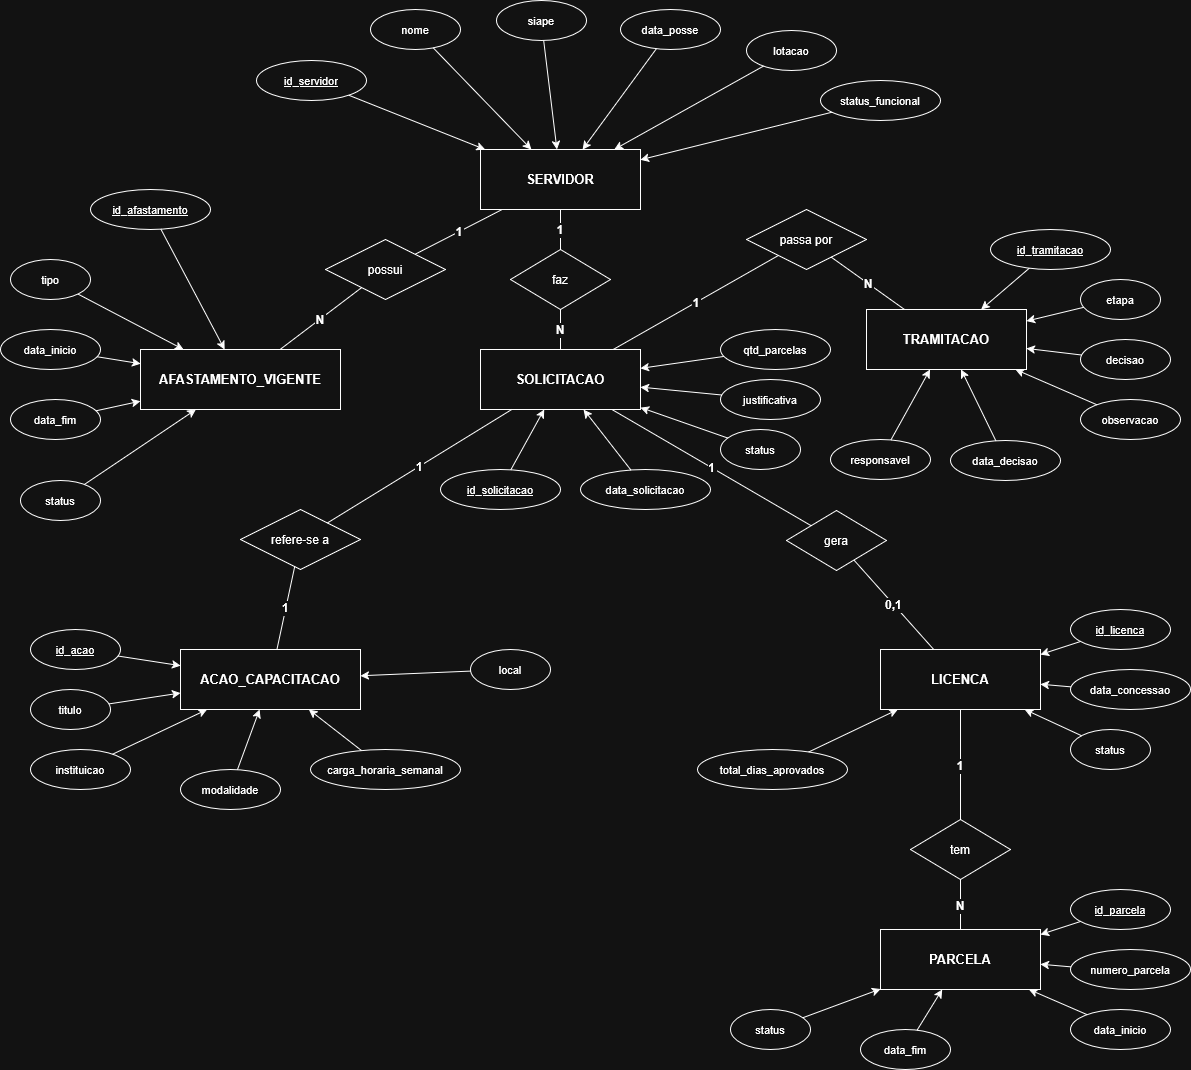
\includegraphics[width=0.95\textwidth]{figuras/der_sistema.png}
\source{Elaborado pelo autor (\imprimirdata).}
\end{figure}

A complexidade algorítmica do módulo de busca foi analisada. A Equação \ref{eq:complexidade} apresenta a complexidade temporal do algoritmo de ordenação utilizado:

\begin{equation}
\label{eq:complexidade}
T(n) = O(n \cdot \log n)
\end{equation}

onde $n$ representa o número de registros a serem ordenados.

\section{Interfaces}

Insira as principais telas do protótipo (\textit{Wireframes} ou \textit{Mockups} de alta fidelidade) desenvolvidas na fase de design. Explique brevemente a funcionalidade de cada tela apresentada.
% ---
% 4 Software
% Este arquivo apresenta o resultado prático do projeto: o software implementado.
% Conforme as Diretrizes do PPC, deve incluir: implantação e testes.
% ---
\chapter{SOFTWARE}
\label{cap:software}

Neste capítulo, o autor deve apresentar o resultado prático do projeto: o software implementado. As Diretrizes do PPC estabelecem que esta seção deve demonstrar o funcionamento do sistema, destacando suas principais funcionalidades através de capturas de tela (\textit{screenshots}) e trechos de código relevantes.

\section{Implantação}

Descreva o processo de implantação (\textit{deploy}) do software. Indique o ambiente de hospedagem utilizado (servidor local, nuvem, etc.), as configurações necessárias e os passos para colocar o sistema em produção.

Apresente as telas do sistema em funcionamento. Diferente da prototipagem (Capítulo \ref{cap:modelagem}), aqui devem ser mostradas as interfaces reais do software finalizado.

\begin{figure}[htb]
\centering
\caption{Tela Inicial do Sistema}
\label{fig:tela_inicial}
% \includegraphics[width=0.9\textwidth]{figuras/tela_inicial.png}
\fbox{\parbox{0.9\textwidth}{\centering \vspace{3cm} [Inserir Print da Tela do Sistema aqui] \\ Salve a imagem em: \texttt{figuras/tela\_inicial.png} \vspace{3cm}}}
\source{Elaborada pelo autor (\imprimirdata).}
\end{figure}

% --- EXEMPLO DE CÓDIGO-FONTE ---
% Utilize o ambiente lstlisting para inserir trechos de código.
% O pacote listings já está configurado em configuracoes.tex.
O Código \ref{lst:codigo_auth} apresenta a função responsável pela autenticação de usuários no sistema.

\begin{lstlisting}[language=Python, caption={Função de autenticação de usuários}, label={lst:codigo_auth}]
from django.contrib.auth.hashers import check_password
from .models import Usuario

def autenticar_usuario(username, password):
    """
    Verifica as credenciais do usuario no banco de dados.
    Retorna o objeto Usuario se autenticado, None caso contrario.
    """
    try:
        usuario = Usuario.objects.get(username=username)
        if check_password(password, usuario.password):
            return usuario
    except Usuario.DoesNotExist:
        pass
    return None
\end{lstlisting}

Explique o funcionamento do código apresentado e como ele se integra ao restante da aplicação. Evite colar trechos excessivamente longos ou gerados automaticamente (como \textit{migrations} ou configurações padrão de \textit{frameworks}); foque na lógica de negócios implementada pelo autor.

% --- EXEMPLO DE ALGORITMO (pseudocódigo) ---
% Para algoritmos em pseudocódigo, utilize o ambiente lstlisting
% com language=none ou crie um estilo customizado.
O Algoritmo \ref{lst:algoritmo_busca} apresenta o pseudocódigo do módulo de busca implementado.

\begin{lstlisting}[caption={Algoritmo de busca por palavra-chave}, label={lst:algoritmo_busca}, language={}]
ALGORITMO BuscaPorPalavraChave
ENTRADA: termo (string), registros (lista)
SAIDA: resultados (lista)

INICIO
    resultados <- lista vazia
    PARA CADA registro EM registros FACA
        SE termo ESTA_CONTIDO_EM registro.titulo OU
           termo ESTA_CONTIDO_EM registro.descricao ENTAO
            ADICIONAR registro EM resultados
        FIM_SE
    FIM_PARA
    ORDENAR resultados POR relevancia DECRESCENTE
    RETORNAR resultados
FIM
\end{lstlisting}

\section{Testes}

Descreva os testes realizados para validar o software. Indique o tipo de teste realizado (unitário, integração, sistema, aceitação, usabilidade) e apresente os resultados obtidos.

\begin{table}[htb]
\centering
\caption{Resultados dos testes realizados}
\label{tab:testes}
\begin{tabular}{@{}llll@{}}
\toprule
\textbf{Código} & \textbf{Tipo} & \textbf{Descrição} & \textbf{Resultado} \\ \midrule
T01 & Unitário & Validação do cadastro de usuário & Aprovado \\
T02 & Unitário & Autenticação com credenciais válidas & Aprovado \\
T03 & Integração & Fluxo completo de login e acesso & Aprovado \\
T04 & Usabilidade & Navegação por usuários leigos & Aprovado \\ \bottomrule
\end{tabular}
\source{Elaborada pelo autor (\imprimirdata).}
\end{table}

% ---
% 5 Considerações Finais
% Este arquivo contém a conclusão do Relatório Técnico de Software.
% Conforme as Diretrizes do PPC, deve retomar os objetivos e discutir
% se foram alcançados, além de apresentar limitações e trabalhos futuros.
% ---
\chapter{CONSIDERAÇÕES FINAIS}
\label{cap:consideracoes}

O capítulo de considerações finais (ou conclusão) deve apresentar uma reflexão sobre o trabalho desenvolvido. Retome os objetivos propostos na Introdução (Capítulo \ref{cap:introducao}) e discuta se foram alcançados.

\section{Resultados Alcançados}

Descreva os principais resultados obtidos com a implementação do software. O sistema resolveu o problema inicial? Como foi a recepção pelos usuários (se aplicável)? Quais foram os maiores desafios enfrentados durante o desenvolvimento e como foram superados?

\section{Limitações do Projeto}

Seja transparente sobre as limitações da versão atual do software. Funcionalidades que foram planejadas mas não puderam ser implementadas devido a restrições de tempo, recursos ou conhecimento técnico devem ser mencionadas aqui.

\section{Trabalhos Futuros}

Sugira melhorias e novas funcionalidades que podem ser adicionadas ao sistema em versões futuras. Esta seção demonstra a visão de longo prazo do autor sobre o produto de software desenvolvido.


% ----------------------------------------------------------
% ELEMENTOS PÓS-TEXTUAIS
% ----------------------------------------------------------
\postextual

% Referências bibliográficas (geradas automaticamente pelo biblatex-abnt)
\printbibliography[heading=bibintoc, title={REFERÊNCIAS}]

% Apêndices (OPCIONAL - descomente se necessário)
% \begin{apendicesenv}
% \partapendices
% \chapter{Documento complementar elaborado pelo autor}
% Insira aqui o conteúdo do apêndice.
% \end{apendicesenv}

% Anexos (OPCIONAL - descomente se necessário)
% \begin{anexosenv}
% \partanexos
% \chapter{Documento externo utilizado como referência}
% Insira aqui o conteúdo do anexo.
% \end{anexosenv}

\end{document}
